% !TeX root = ../main.tex
\chapter{Simulation Results}
\label{chap:simulations}

\begin{weekthreechange}
    \st{No simulations were performed for this project; instead, calculations were performed, and preliminary tests carried out with an evaluation board.}

    Simulations were performed using LTSpice in a DC Operating Point simulation to verify the calculation for the full-load shunt voltage for each of the voltages. Only the positive polarity was tested in the simulation, as negative polarity will naturally not matter to a a passive element such as the resistor.

    The data collected in this simulation matches the data found in Appendix A section \ref{sec:shunt-sizing}, table \ref{tab:production-shunts}

    \begin{figure}[H]
        \centering
        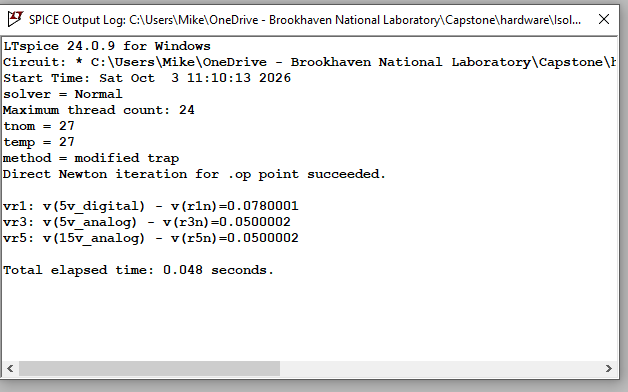
\includegraphics[
        width=.85\textwidth,
        %height=0.85\textwidth,
        keepaspectratio
        ]{Pictures/SimulationResultsLog}
        \caption{Simulation verifying current shunt voltage drops, data log}
    \end{figure}

\end{weekthreechange}

\clearpage

\begin{sidewaysfigure}[p]
    \centering
    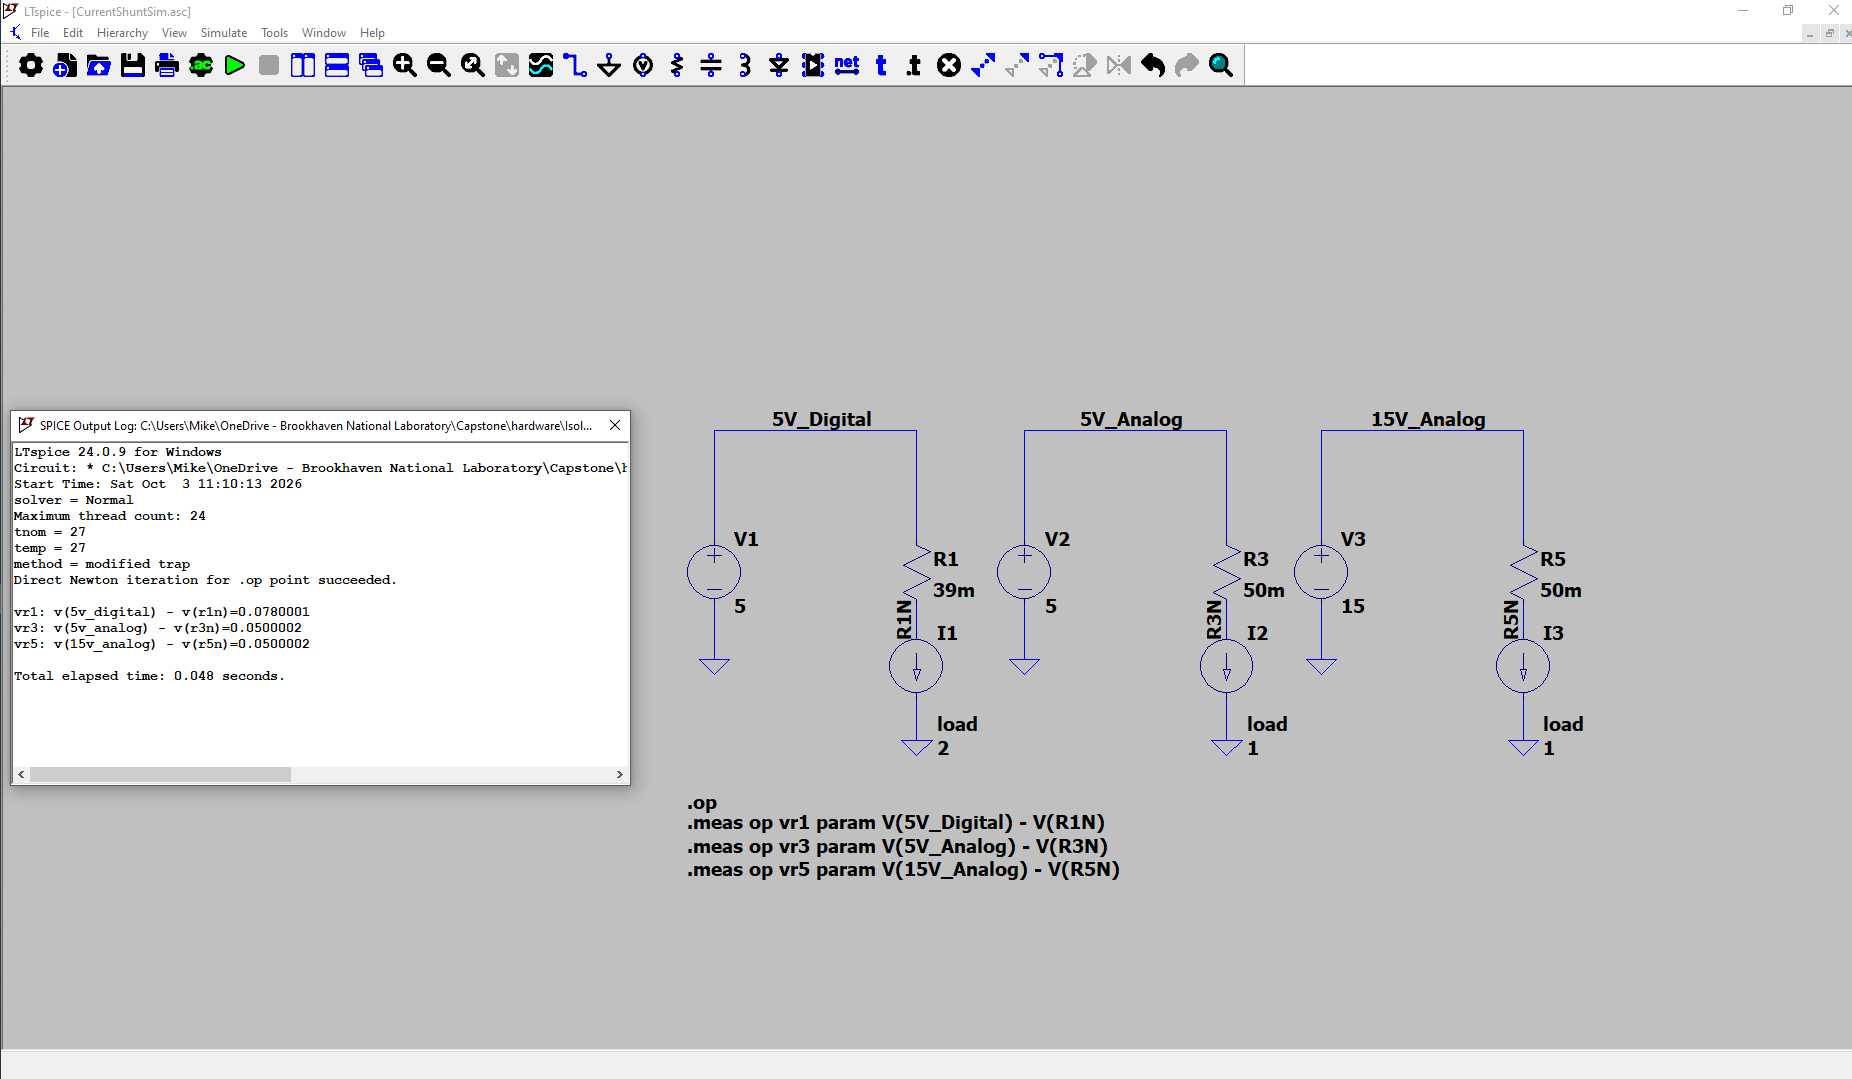
\includegraphics[
    width=0.95\textheight,
    keepaspectratio
    ]{Pictures/SimulationResults}
    \caption{Simulation verifying current shunt voltage drops, full simulation screenshot}
    \label{fig:SimulationResults}
\end{sidewaysfigure}
